\documentclass[12pt,a4paper,portuguese]{article}
\usepackage[T1]{fontenc}
\usepackage{babel}
\usepackage{graphicx}
\usepackage{float}
\usepackage{pythonhighlight}

\title{Lista 2 - Análise de Séries Temporais em Oceanografia}
\author{Lucas Salimene}
\date{}
\begin{document}
	\maketitle
	\newpage
	\textbf{Parte I – Teorema do Limite Central}
	Gerando a série aleatória com o código:
	\begin{python}
a=1
n=3000
b=100
x = a*np.random.normal(size=n)+b
	\end{python}
O modo padrão do random do Numpy já está configurado para ser equivalente ao modo "twister" do MATLAB, com isso, é possível obter a média, variância e desvio padrão conforme a tabela \ref{xmvstd}
\begin{table}[H]
\centering
\begin{tabular}{|c|c|}
	\hline
	Média & 99.99 \\
	\hline
	Variância & 1.03 \\
	\hline
	Desvio Padrão & 1.01 \\
	\hline
\end{tabular}
\caption{Média, Variância e Desvio padrão da série aleatória}
\label{xmvstd}
\end{table}
Utilizando a rotina \textcolor{red}{make$\_$segments.m} adaptada para Python, foi possível segmentar a série, a figura \ref{fig:lista2-1c} mostra os histogramas da série segmentada e da série original
\begin{figure}[H]
	\centering
	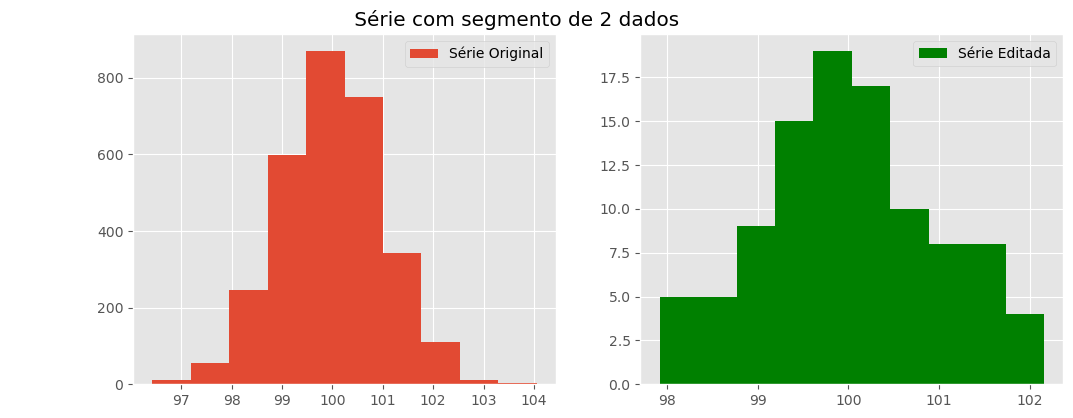
\includegraphics[width=0.9\linewidth]{lista2-1c}
	\caption{Histograma das séries aleatórias. \textbf{Esquerda} série original. \textbf{Direita} série segmentada}
	\label{fig:lista2-1c}
\end{figure}
	\begin{table}[H]
		\centering
		\begin{tabular}{|c|c|}
			\hline
			Média & 99.99 \\
			\hline
			Variância & 1.02 \\
			\hline
			Desvio Padrão & 1.01 \\
			\hline
		\end{tabular}
		\caption{Média, Variância e Desvio padrão da série segmentada}
		\label{y2}
	\end{table}
Repetindo o processo para segmentos de 5 e 30:

\begin{figure}[H]
	\centering
	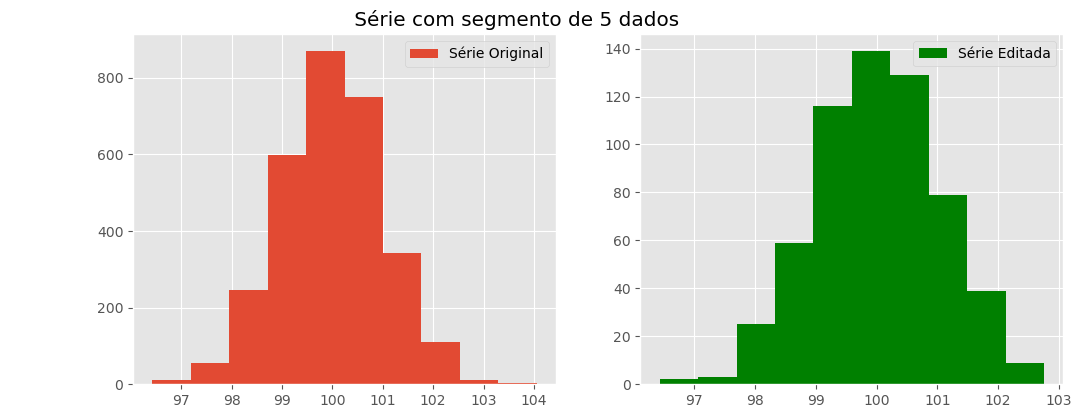
\includegraphics[width=0.9\linewidth]{lista2-1d}
	\caption{Histograma das séries aleatórias. \textbf{Esquerda} série original. \textbf{Direita} série segmentada em segmentos de 5 dados}
	\label{fig:lista2-1d}
\end{figure}


\begin{figure}[H]
	\centering
	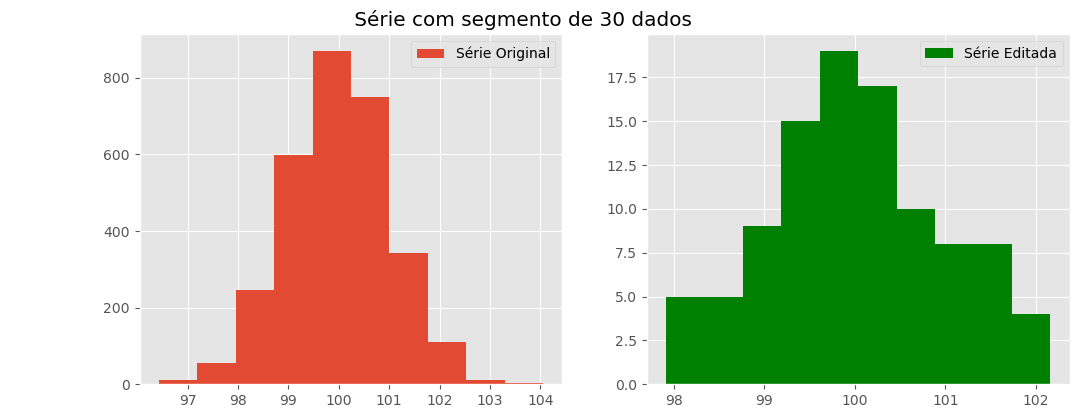
\includegraphics[width=0.9\linewidth]{lista2-1e}
	\caption{Histograma das séries aleatórias. \textbf{Esquerda} série original. \textbf{Direita} série segmentada em segmentos de 30 dados}
	\label{fig:lista2-1e}
\end{figure}
Como se observa pelas figuras \ref{fig:lista2-1c},\ref{fig:lista2-1d} e \ref{fig:lista2-1e}, as séries visualmente se assemelham a uma distribuição normal.
Repetindo para:
\begin{python}
a=1
n=3000
b=100
x = a*np.random.sample(size=n)+b
\end{python}
\begin{figure}[H]
	\centering
	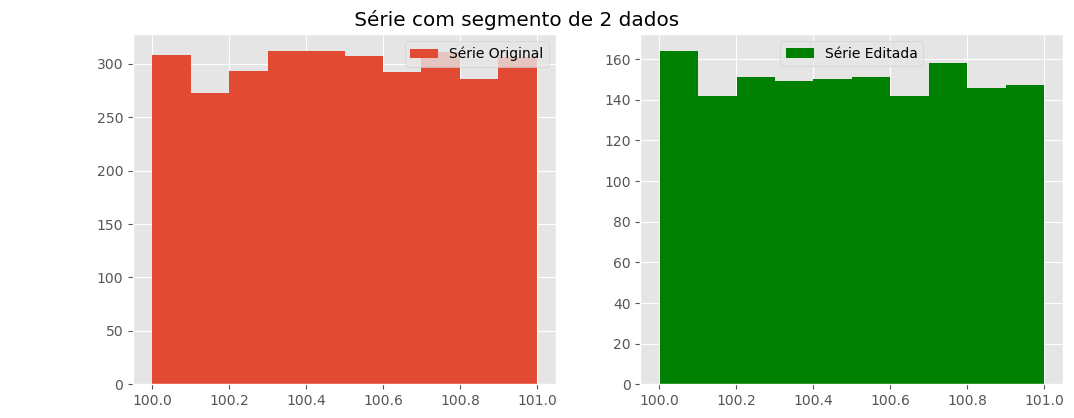
\includegraphics[width=0.9\linewidth]{lista2-2c}
	\caption{Histograma das séries aleatórias. \textbf{Esquerda} série original. \textbf{Direita} série segmentada}
	\label{fig:lista2-2c}
\end{figure}
\begin{table}[H]
	\centering
	\begin{tabular}{|c|c|}
		\hline
		Média & 100.5 \\
		\hline
		Variância & 0.08 \\
		\hline
		Desvio Padrão & 0.28 \\
		\hline
	\end{tabular}
	\caption{Média, Variância e Desvio padrão da série segmentada}
	\label{y2}
\end{table}
	
	\begin{figure}[H]
		\centering
		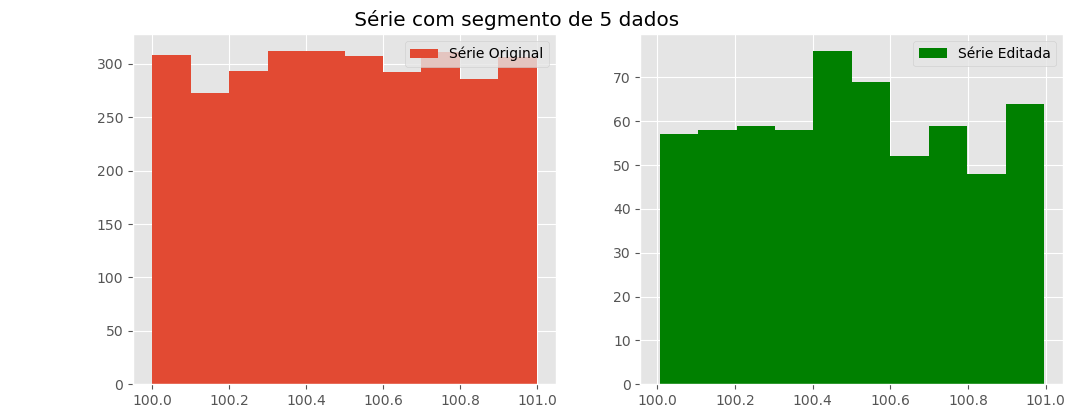
\includegraphics[width=0.9\linewidth]{lista2-2d}
		\caption{Histograma das séries aleatórias. \textbf{Esquerda} série original. \textbf{Direita} série segmentada em segmentos de 5 dados}
		\label{fig:lista2-2d}
	\end{figure}
	
	
	\begin{figure}[H]
		\centering
		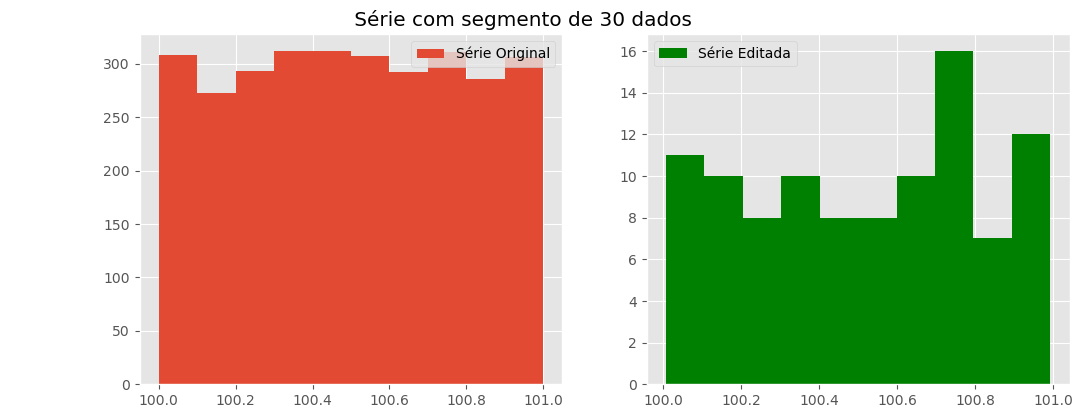
\includegraphics[width=0.9\linewidth]{lista2-2e}
		\caption{Histograma das séries aleatórias. \textbf{Esquerda} série original. \textbf{Direita} série segmentada em segmentos de 30 dados}
		\label{fig:lista2-2e}
	\end{figure}
	
	
	Repetindo para:
	\begin{python}
a=1
n=3000
b=100
x = np.exp(-np.arange(1, n+1)/1000)
	\end{python}
	\begin{figure}[H]
		\centering
		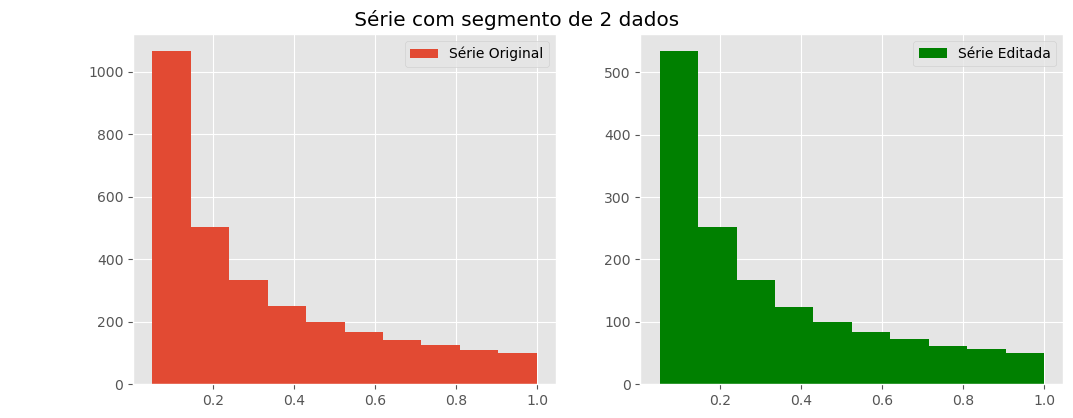
\includegraphics[width=0.9\linewidth]{lista2-3c}
		\caption{Histograma das séries aleatórias. \textbf{Esquerda} série original. \textbf{Direita} série segmentada}
		\label{fig:lista2-3c}
	\end{figure}
	\begin{table}[H]
		\centering
		\begin{tabular}{|c|c|}
			\hline
			Média & 0.32\\
			\hline
			Variância & 0.06\\
			\hline
			Desvio Padrão &0.26\\
			\hline
		\end{tabular}
		\caption{Média, Variância e Desvio padrão da série segmentada}
		\label{y2}
	\end{table}
	
	\begin{figure}[H]
		\centering
		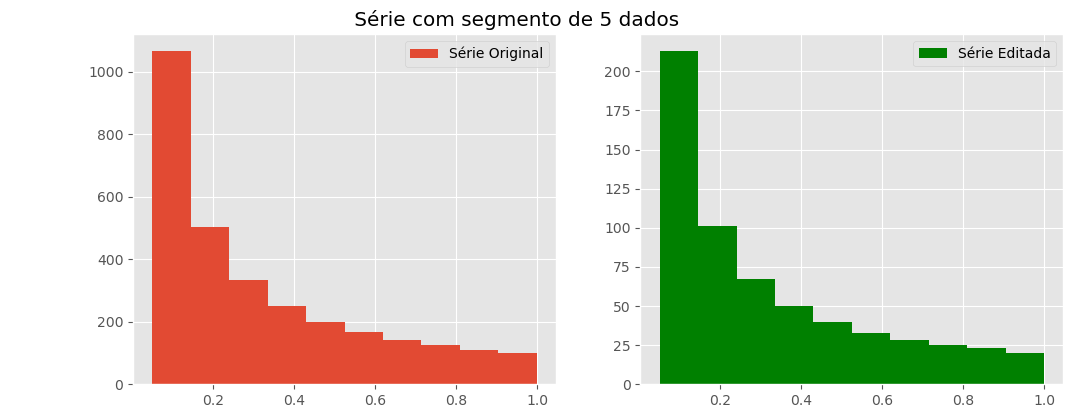
\includegraphics[width=0.9\linewidth]{lista2-3d}
		\caption{Histograma das séries aleatórias. \textbf{Esquerda} série original. \textbf{Direita} série segmentada em segmentos de 5 dados}
		\label{fig:lista2-3d}
	\end{figure}
	
	
	\begin{figure}[H]
		\centering
		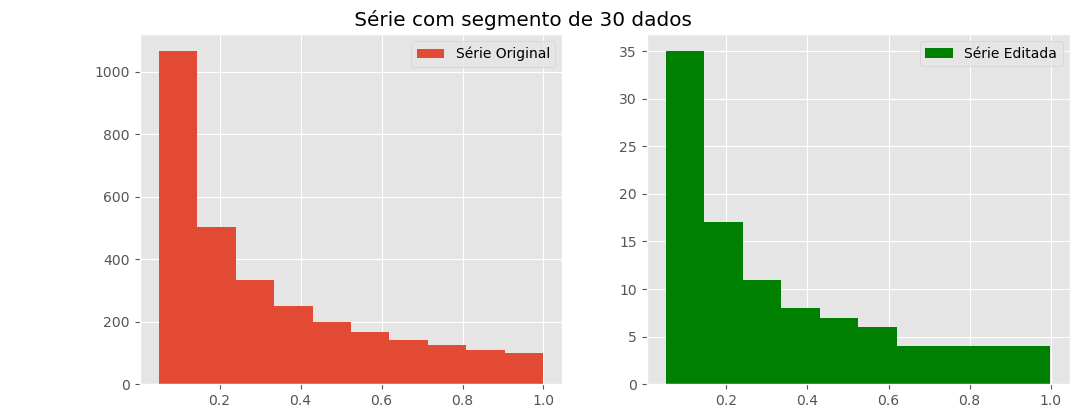
\includegraphics[width=0.9\linewidth]{lista2-3e}
		\caption{Histograma das séries aleatórias. \textbf{Esquerda} série original. \textbf{Direita} série segmentada em segmentos de 30 dados}
		\label{fig:lista2-3e}
	\end{figure}
	
	\textbf{Parte II – Teste de Estacionaridade}
	
Utilizando os dados do arquivo SST.mat recordados nos primeiros 2000 pontos, foi feito a interpolação linear e a utilizando dos
	
\end{document}